Die gewohnte Bewegungsfreiheit in der erweiterten Realität beizubehalten ist bei weitem nicht trivial.
Zwar ist der Körper nicht eingeschränkt und es kann problemlos durch die durchsichtigen Gläser von AR--Headsets gesehen werde, allerdings bewegt sich der Ursprung des bekannten Koordinatensystems.

Die schwierigkeit liegt also darin, Objekte im realen Raum platzieren zu können.
\footnote{Ein weiteres großes problem, mit dem wir uns an dieser Stelle nicht befassen wollen, ist die Interaktion mit diesen objekten, also das Body Tracking.}

\subsection{Degrees Of Freedom}\label{subsec:degrees-of-freedom}
    Degrees Of Freedom~\autocite{wikipedia-contributors-2023B}, kurz \textbf{DOF}, bezeichnen die Bewegungsfreiheiten eines Systems in einem Vektorraum.
    Ein einfaches Beispiel sei mit der klassischen Transformationsmatrix in \autoref{fig:matrix-DOFs} gegeben.

    \begin{figure}[ht!]
        \begin{center}
            \begin{math}
                \begin{bmatrix}
                {\color{red} s}
                    \cdot {\color{green} t_{1,1}} & {\color{green} t_{1,2}}                       & {\color{green} t_{1,3}}                       & {\color{blue} v_x} \\
                    {\color{green} t_{2,1}}       & {\color{red} s} \cdot {\color{green} t_{2,2}} & {\color{green} t_{2,3}}                       & {\color{blue} v_y} \\
                    {\color{green} t_{3,1}}       & {\color{green} t_{3,2}}                       & {\color{red} s} \cdot {\color{green} t_{3,3}} & {\color{blue} v_z} \\
                    0                             & 0                                             & 0                                             & {\color{red} s}
                \end{bmatrix}
            \end{math}
        \end{center}
        \begin{tabular}{c|c|c}
            var             & Bezeichnung & DOF \\
            \hline
            \color{red} s   & Skalar      & 1   \\
            \color{blue} v  & Vektor      & 3   \\
            \color{green} t & Tensor      & 6   \\
        \end{tabular}
        \caption{Degrees Of Freedom der Transformationsmatrix}
        \label{fig:matrix-DOFs}
    \end{figure}

    Ein degree of freedom bezeichnet dabei einen eindimensionalen Parameter des Systems.
    Es wird also mit jedem Parameter ein größerer Vektorraum aufgespannt.
    Der degree of freedom entspricht damit der Dimension des zugehörigen Vektorraumes.

    Der visuell einfachste Teilraum aus \autoref{fig:matrix-DOFs} ist das kartesische Koordinatensystem, hier bezeichnet als \textbf{Vektor}.
    Im dreidimensionalen Raum ist eine Bewegung in 3 Richtungen möglich.

    Dazu kommt die \textbf{Skalierung}.
    Auch diese sollte leicht verständlich sein.

    Komplizierter wird die \textbf{Tensor}-Transformation.
    Diese bezeichnet die Kombination aus \textbf{Rotation} und \textbf{Scherung}.
    Diese sind jeweils um alle 3 Achsen des kartesischen Koordinatensystems möglich und haben damit jeweils 3~DOF\@.
    Daraus ergeben sich 10~DOF der klassischen Transformationsmatrix.

    AR--Headsets sind allerdings deutlich eingeschränkter.
    Sie haben 6~DOF~\autocite{wikipedia-contributors-2023B}.

    Das physische Headset kann sich, wie in \autoref{fig:6DOF} dargestellt, im Raum von $\vec{a}$ nach $\vec{b}$ bewegen und um jede seiner Achsen rotieren, allerdings nicht geschert oder skaliert werden.

    \begin{figure}[ht!]
        \center
        \includesvg[width={0.5\textwidth}]{../assets/img/6DOF}
        \caption{6 Degrees Of Freedom~\autocite{wikipedia-contributors-2023B}}
        \label{fig:6DOF}
    \end{figure}

    Damit wird die Darstellung meistens auf einen Vektor für die Position sowie eine Quaternion~\autocite{wikipedia-contributors-2023G} für die Rotation beschränkt.

\subsection{Positioning System}\label{subsec:positioning-system}
    Das bringt die Entwicklung von AR--Headsets vor seine ganz eigene Herausforderung, da diese 6~DOF notwendig sind, um dem nutzer ein minimum an Orientierung zu bieten.

    Dazu werden Positionierungssysteme~\autocite{wikipedia-contributors-2023A} verwendet.

    \subsubsection{Global Positioning System}\label{subsubsec:global-positioning-system}
        Eines der bekanntesten Positionierungssysteme ist das GPS~\autocite{wikipedia-contributors-2023J}, welches heutzutage in jedem Mobiltelefon verbaut ist.
        GPS ist eines der wenigen globalen Satellitennavigationssysteme.

        Diese Systeme lösen das Problem der Positionierung, wie der Name suggeriert, indem, mindestens 4, Satellite, in Sichtweite, Radiowellen aussenden.
        Die Radiowellen tragen als Signal den Zeitstempel des senden des Signals.
        Damit ist der Abstand vom Empfänger zum Sender von allen Satellite in Sichtweite bekannt.

        \begin{figure}[ht!]
            \center
            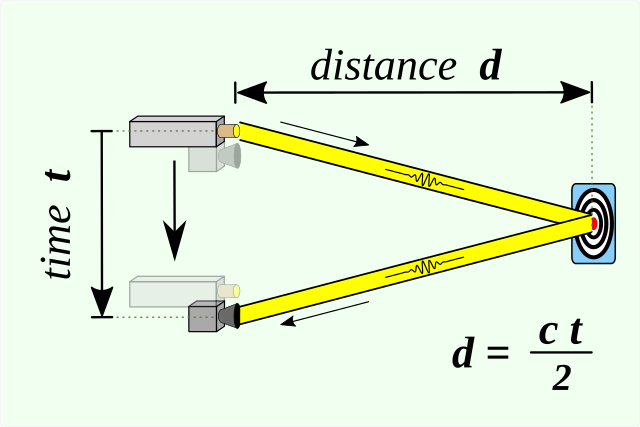
\includegraphics[width={0.5\textwidth}]{../assets/img/time_of_flight}
            \caption{Time of Flight~\autocite{wikipedia-contributors-2023D}}
            \label{fig:ToF}
        \end{figure}

        Dieses Konzept wird Time of Flight~\autocite{wikipedia-contributors-2023D}, kurz \textbf{ToF}, genannt und ist in \autoref{fig:ToF} dargestellt.

        Für jeden degree of freedom wird allerdings mindestens ein Parameter benötigt.
        Deshalb können aus den 4 Zahlen auch nur 3~DOF, also die Position, auf 0.3 bis zu 5 Meter genau, errechnet werden.

    \subsubsection{Indoor Positioning System}\label{subsubsec:indoor-positioning-system}
        Aufgrund dieser Ungenauigkeit kann GPS auch nicht für die ersten 3~DOF genutzt werden.
        Auch mit 30~cm ungenauigkeit könnten wir in keine virtuelle Realität eintauchen.

        Deshalb müssen genauere Systeme her, sogenannte Indoor Positioning Systems~\autocite{wikipedia-contributors-2023E}.
        Diese sind Systeme, die die Positionierung innerhalb eines Raums oder Arbeitsplatzes ermöglichen.
        Ob 6~DOF oder lediglich 3~DOF erreicht werden ist dabei vom jeweiligen System abhängig.

        \paragraph{Base Stations}\label{par:base-stations} werden hierfür klassischerweise verwendet.
            Diese sind externe Geräte, welche, ähnlich wie die Satellite beim GPS, die Position des Empfängers ermitteln.

            Es gibt einige enterprise Systeme, welche zum Beispiel in Lagerhäusern verwendet werden.\footnote{Allerdings gibt es mittlerweile auch hybride Systeme, welche die in \autoref{subsubsec:spatial-anchors} beschriebenen Systeme mit einbeziehen.~\autocite{he-2021}}~\autocite{wikipedia-contributors-2023E}
            Für diese Ausarbeitung werden wir uns allerdings als Beispiel die SteamVR Base Station 2.0~\autocite{valve-corporation-no-date} anschauen.

            Diese nutzen allerdings keine Time of Flight.
            Anstatt die Position aus der Distanz zu errechnen wird hier die Position durch das Abtasten mittels eines Lasers ermittelt.
            Damit werden mehrere markante Punkte an dem VR-Headset pro Basisstation abgetastet.
            Es ergeben sich daraus also 6~DOF\@.

        \paragraph{Spatial cognition}~\autocite{wikipedia-contributors-2023F} ist die Warnehrung der Umgebung vom Menschen und anderen Lebewesen.
            Unter anderem umfasst dieses Thema die Objektpermanenz.

            Als ein bionischer Ansatz wird dieses Konzept heute auf AR--Headsets angewendet.
            Daraus ergeben sich 6~DOF, ohne an einen zuvor eingerichteten Raum gebunden zu sein.
            Die funktionalität solcher Systeme ist in \autoref{subsec:spatial-cognition-fuer-ar-headsets} beschrieben.

\subsection{Spatial Cognition beim Menschen}\label{subsec:spatial-cognition-beim-menschen}
    Das Kernkonzept der Spatial Cognition ist das Verarbeiten von Wissen über die Umgebung. \autocite{wikipedia-contributors-2023F}
    Es wird dabei regelmäßig neu organisiert, um das Verständnis der Umwelt zu verbessern.

    Als ein Beispiel wollen wir uns anschauen, wie Menschen ihre Umgebung beschreiben.
    Die wahrnehmung der Umgebung, spezieller ihre Darstellung, wie in \autoref{subsubsec:cognitive-map} weiter beschrieben, wird weitestgehend von der Sprache beeinflusst. \autocite{haviland-1998}
    Ich, so wie die meisten Leser vermutlich auch, sehe vor mir meinen Laptop, an dem ich dieses Paper schreibe.
    Für einen Sprecher der indigenen Sprache Guugu Yimithirr wäre mein Laptop südöstlich von mir.
    Das heißt, für uns ist die eigene Orientierung im Raum wichtiger für die eigene Wahrnehmung.

    Um kurz in die Computergrafik zurückzukehren, ein Vergleich wäre das World Coordinate System für uns und das Camera Coordinate System für Guugu Yimithirr sprecher.

    Wir versetzen uns gerne in andere hinein, das ist aber ungünstig für Jagen oder Kämpfen in einer Formation.
    Während die Spatial Cognition bei Lebewesen zahlreiche Fachbereiche der Biologie und Psychologie abdeckt, stellt sich für uns die Frage, welche Informationen für den Nutzer am wichtigsten sind, um nicht die Orientierung zu verlieren, sowie welche Darstellungsformen wir übernehmen können, um die klassische Transformationsmatrix dieses Systems zu befähigen.

    \subsubsection{Navigation}\label{subsubsec:navigation}
        Diese beiden Systeme nennt man \enquote{Egocentric Navigation}\footnote{Beschreiben aus der Ich--Perspektive} und \enquote{Allocentric Navigation}\footnote{Beschreiben von einem allgemeinen Referenzpunkt}.~\autocite{wikipedia-contributors-2023F}

        Zum Navigieren in großen, unbekannten Umgebungen ist dabei die Allocentric Navigation von Vorteil.
        Es werden große Referenzpunkte in der Landschaft gesucht und anhand eines globalen Koordinatensystems (Kompass) Richtungen angegeben.
        Die Abdeckung der Navigation ist damit höher.

        In bekannten Umgebungen ist die Egocentric Navigation allerdings im Vorteil.
        Vor allem lokale Objekte und der Navigierende selbst werden als Referenz verwendet zusammen mit relationalen Begriffen wie \enquote{Links} oder \enquote{Rechts}.
        Da sich nicht so viele Sachen gemerkt werden müssen ist diese Art der Navigation effizienter, auf kosten der Effektivität.

    \subsubsection{Proprioception}\label{subsubsec:proprioception}
        Proprioception ist die Wahrnehmung des eigenen Körpers. \autocite{wikipedia-contributors-2023H}
        Spezifischer: die Wahrnehmung der eigenen Muskeln.

        Dadurch, dass die Ausdehnung jedes Muskels im Körper bekannt ist, wissen wir auch mit geschlossenen Augen, wo z.B.\ unser Arm ist.

        Diese Informationen fließen über das zentrale Nervensystem entweder in das Bewusstsein oder das Unterbewusstsein.
        Hier wird aus diesen Informationen, zusammen mit den anderen Sinnen, wie z.B.\ Sehen, Hören, Riechen oder der Gleichgewichtssinn; eine \enquote{Karte} von unserer Umgebung und unserer Körperposition erstellt.

    \subsubsection{Cognitive Map}\label{subsubsec:cognitive-map}
        Diese Cognitive Maps~\autocite{wikipedia-contributors-2023I} nutzen das sogenannte \enquote{Spatial Knowledge}, also all die zuvor beschriebenen Informationen, und bilden daraus eine abstrakte Darstellung.
        Diese wird umgangssprachlich manchmal als inneres Auge bezeichnet.

        \enquote{Map} ist hierbei nicht als Karte zu verstehen, sondern als Abbildung.
        Auch wenn es das anschaulichste Beispiel ist, weshalb wir uns in dieser Arbeit darauf begrenzen, können jegliche informationen auf diese Art und Weise abstrakt dargestellt werden.

        Handelt es sich um eine karten--ähnliche Struktur, so setzt sie sich, unter anderem, aus zwei Arten von Information zusammen:
        \begin{enumerate}
            \item Positional Landmarks\\
            Landmarks, oder Referenzpunkte, geben einen Uhrsprung für Wissen über die Umgebung.
            \item Directional Cues\\
            Richtungsangaben spezifizieren Relationen zwischen Objekten.
        \end{enumerate}

    \subsubsection{Reference Frames}\label{subsubsec:reference-frames}
        In \autoref{subsubsec:navigation} haben wir die Begriffe \enquote{Egocentric Navigation} und \enquote{Allocentric Navigation} kennen gelernt.
        Jetzt wollen wir diese Begriffe etwas verallgemeinern, damit wir sie später auch mittels Software formalisieren können.

        Um sich im Raum zurechtzufinden, also Spatial Knowledge zu besitzen, muss es immer einen Referenzpunkt~\autocite{wikipedia-contributors-2023F}, genauer ein Referenzkoordinatensystem geben.
        Wir wissen bereits, dass diese Referenz die Ich--Perspektive\footnote{Beim Menschen ist es die Egocentric Navigation, in der VR sind es HUDs}, signifikante Punkte in der Landschaft\footnote{Beim Menschen ist es die Allocentric Navigation, in der VR sind es Base Stations} oder das Magnetfeld der Erde\footnote{Beim Menschen ist es der Kompass, in der Technik GPS} sein können.
        Dies sind aber nicht die einzigen Optionen.

        Ein nennenswertes Problem ist die Navigation im Weltraum.
        Hier wird meistens ein Gitter mit einem frei gewählten Nullpunkt verwendet.

        Allerdings ist das Referenzsystem beim Menschen dynamisch und individuell.
        Auch wenn nur wenige formularisiert sind, so gibt es sehr viele mehr.

\subsection{Spatial Cognition für AR--Headsets}\label{subsec:spatial-cognition-fuer-ar-headsets}
    In \autoref{subsec:degrees-of-freedom} haben wir uns die Transformationsmatrix aus der klassischen Computergrafik angeschaut.
    Diese basiert auf einem klassischen, 3--dimensionalen, kartesischen Koordinatensystem.
    Da das klassische Sichtvolumen definiert ist, durch $S=\left\{(x,y,z)\in \mathbb{R}^3;-1\leq x\leq 1\land -1\leq y\leq 1\land -1\leq z\leq 1\right\}$, liegt der Mittelpunkt auf dem Ursprung des Koordinatensystems.

    Übertragen wir diese Information auf den Bildschirm vor dem Gesicht des Nutzers eines AR--Headsets, so ergibt sich daraus eine \enquote{Egocentric Navigation}, bzw.\ ein egozentrisches Koordinatensystem.
    Es können also, ohne das Rad neu zu erfinden, Objekte in relativer Position zum Nutzer platziert werden.

    So kann sich der Nutzer allerdings nicht durch diese virtuelle Welt bewegen.
    Es sind 0~DOF\@.

    Es wird also eine \enquote{Allocentric Navigation}, bzw.\ ein allozentrisches Koordinatensystem, benötigt, um tatsächlich Bewegungsfreiheit (degrees of freedom) zu ermöglichen.

    \subsubsection{World Coordinate System}\label{subsubsec:world-coordinate-system}
        Um diese \enquote{Allocentric Navigation} zu erreichen wird ein globales Koordinatensystem eingeführt, das \enquote{World Coordinate System}~\autocite{sean-kerawala-2022}.

        Dies ist das standard Koordinatensystem, welches aus der klassischen Render--Pipeline bekannt ist.
        Damit wird das Egozentrische--Koordinatensystem zu unserem Kamera--Koordinatensystem.

        Per Konvention ist in diesem Koordinatensystem die Einheit 1m.

        Der große Unterschied zum normalen Rendering ist, dass die Kamera nicht vom Programm, sondern vom Nutzer, bewegt wird.

        Allerdings fehlt uns immer noch ein IPS, wie in \autoref{subsubsec:indoor-positioning-system} beschrieben.

    \subsubsection{Knowledge engineering}\label{subsubsec:knowledge-engineering}
        Hier kommt Knowledge engineering ins Spiel:\\
        Wir brauchen ein sogenanntes \enquote{Knowledge--based System}.~\autocite{wikipedia-contributors-2023C}

        Dies sind systeme, die strukturiertes Wissen, also ein semantisches Netzwerk~\autocite{wikipedia-contributors-2023K}, verwalten und zugänglich machen.

        Dieses Wissen kommt aus den Sensoren des AR--Headsets, beispielsweise der Kamera oder dem Gyroskop.
        Die Daten werden jeden Frame ausgewertet und anhand der aktuellen, bekannten Position im World Coordinate System, dem semantischen Netzwerk hinzugefügt.
        Somit entsteht ein Netzwerk aus Referenzpunkten, oder \enquote{Positional Landmarks} (Siehe \autoref{subsubsec:cognitive-map},) die die Umgebung beschreiben.

        \paragraph{D}amit fehlt nicht mehr viel zu einem Indoor Positioning System.
            Die Wissensbasis der Referenzpunkte kann analog zu den Base Stations verwendet werden, um die Position auszumachen.
            Die Rotation kann anschließend durch das Gyroskop einfach gemessen werden.

        \paragraph{V}orraussetzung dafür, ein solches System überhaupt mit Daten füllen zu können ist allerdings eine effiziente Auswertung der Sensordaten.
            Hierzu werden Heuristika oder spezifischer meist künstliche Intelligenz verwendet.
            Da diese meist auch effizient auf der GPU laufen, konkurrieren sie mit der hohen Grafikanforderung an AR--Headsets.
            Mehr dazu in \autoref{subsec:renderpipeline-der-hololens2}.

    \subsubsection{Spatial anchors}\label{subsubsec:spatial-anchors}
        Ein System, welches auf diese Art und Weise ein IPS umsetzt sind Microsofts Spatial Anchors.~\autocite{thetuvix-2023B}

        Deren AR--Headsets, die Hololens2, nutzt dieses System.
        Allerdings bietet dieses System auch die möglichkeit, einzelne, oder auch alle, Referenzpunkte mit anderen Geräten zu teilen.
        Damit können dann sogar Objekte zwischen zwei (oder mehreren) AR--Headsets geteilt werden.~\autocite{pamistel-2022}
        Wir beschränken uns aber auf den einsatz des Systems auf einer Hololens2, da wir uns mit dem Computer--grafischen Teil des Systems befassen wollen.

        Ein Spatial Anchor ist, zusätzlich zu seiner Funktion als Referenzpunkt für das IPS, sein eigenes Koordinatensystem.
        In diesem können Objekte platziert werden, welche dann relativ zu dem Referenzpunkt besonders stabil positioniert sind.
        Diese werden anschließend beim Rendern in das World Coordinate System transformiert.

        Allerdings werden sie auch erste beim Rendern in das World Coordinate System übertragen.
        Sie werden immer wieder neu in relation zueinander positioniert.
        Dies hat den vorteil, dass sie genauer ihre Position in der echten Welt behalten.

        Wenn nicht unter der Haube vom System, werden Spatial Anchors meistens von Nutzern erstellt.
        Zum Beispiel, wenn ein nutzer mittels des Gaze\footnote{Als Gaze bezeichnet Microsoft das Equivalent eines Cursors zur Interaktion im 3--dimmensionalen Raum. Auf der Hololens ist es eine Linie, die den Punkt markiert, auf den der Nutzer schaut und auf der HoloLesn2 ist es der Punkt,auf den der nutzer mittels einem beliebigen seiner Zeigefinger zeigt.~\autocite{sostel-2023} Unter der Haube findet dafür ein Raycast stadt. Mittels des Spatial Mappings kann der Raycast auch reale Objekte treffen.~\autocite{mattzmsft-2023}} ein Objekt platziert.
        Wie in \autoref{lst:place-spatial-anchor} dargestellt, wird zunächst am nächsten, umliegenden, signifikanten Punkt, oder Landmark, ein Spatial Anchor erstellt, in dessen Koordinatensystem anschließend das Objekt platziert wird.

        \lstinputlisting[label={lst:place-spatial-anchor},caption={Platzieren eines Spatial Anchors nach Nutzerinteraktion (Pseudocode)},language=Kotlin]{../assets/code/place_spatial_anchor.kt}

        Dadurch ist das erstellte Objekt für den Nutzer an den Ort gebunden, an welchem er das Objekt platziert hat.

        \paragraph{N}achteil dieses Systems ist die Winkelungenauigkeit.
            Da der Fehler der Spatial Anchors größer wird, desto weiter der Nutzer sich entfernt, sollten Objekte maximal 3~Meter vom Uhrsprung eines Spatial Anchors platziert werden.
            Sie können also nicht für dynamische\footnote{in einem großen Umkreis, viel bewegte} Objekte verwendet werden.

    \subsubsection{Stationary frame of reference}\label{subsubsec:stationary-frame-of-reference}
        Auch ohne das Koordinatensystem eines Spatial Anchors können Objekte platziert werden.
        Mittels des \enquote{stationary frame of reference}~\autocite{thetuvix-2023A} können auch Objekte im World Coordinate System platziert werden.
        Diese Objekte werden dann als \enquote{World--Locked} bezeichnet.

        Da der stationary frame of reference allerdings von den Spatial Anchors als IPS abhängig ist und bei der Vermessung zwischen verschiedenen Spatial Anchors heute noch signifikante Fehler entstehen ist die nutzung nicht in einer großflächigeren Nutzungsumgebung empfohlen.
        Microsoft empfiehlt ein Limit von 5~Metern.

        Für sogenannte \enquote{world--scale experience} muss eine kombination aus den 3 Typen von Koordinatensystemen genutzt werden.
        Wir kategorisieren also in HUD, world--locked und anchored positionierte Objekte.

\subsection{Render--Pipeline der Hololens2}\label{subsec:renderpipeline-der-hololens2}
    Da Informationen zu diesem Thema weitestgehend unveröffentlicht sind, handelt es sich im Folgenden um begründete Vermutungen.

    In \autoref{subfig:render-pipeline-classic} ist, grob vereinfacht, die Render--Pipeline einer klassischen Grafikanwendung dargestellt.
    Spannend für uns ist die Vertex--Verarbeitung.

    \begin{figure}[ht!]
        \begin{subfigure}{0.5\textwidth}
            \centering
            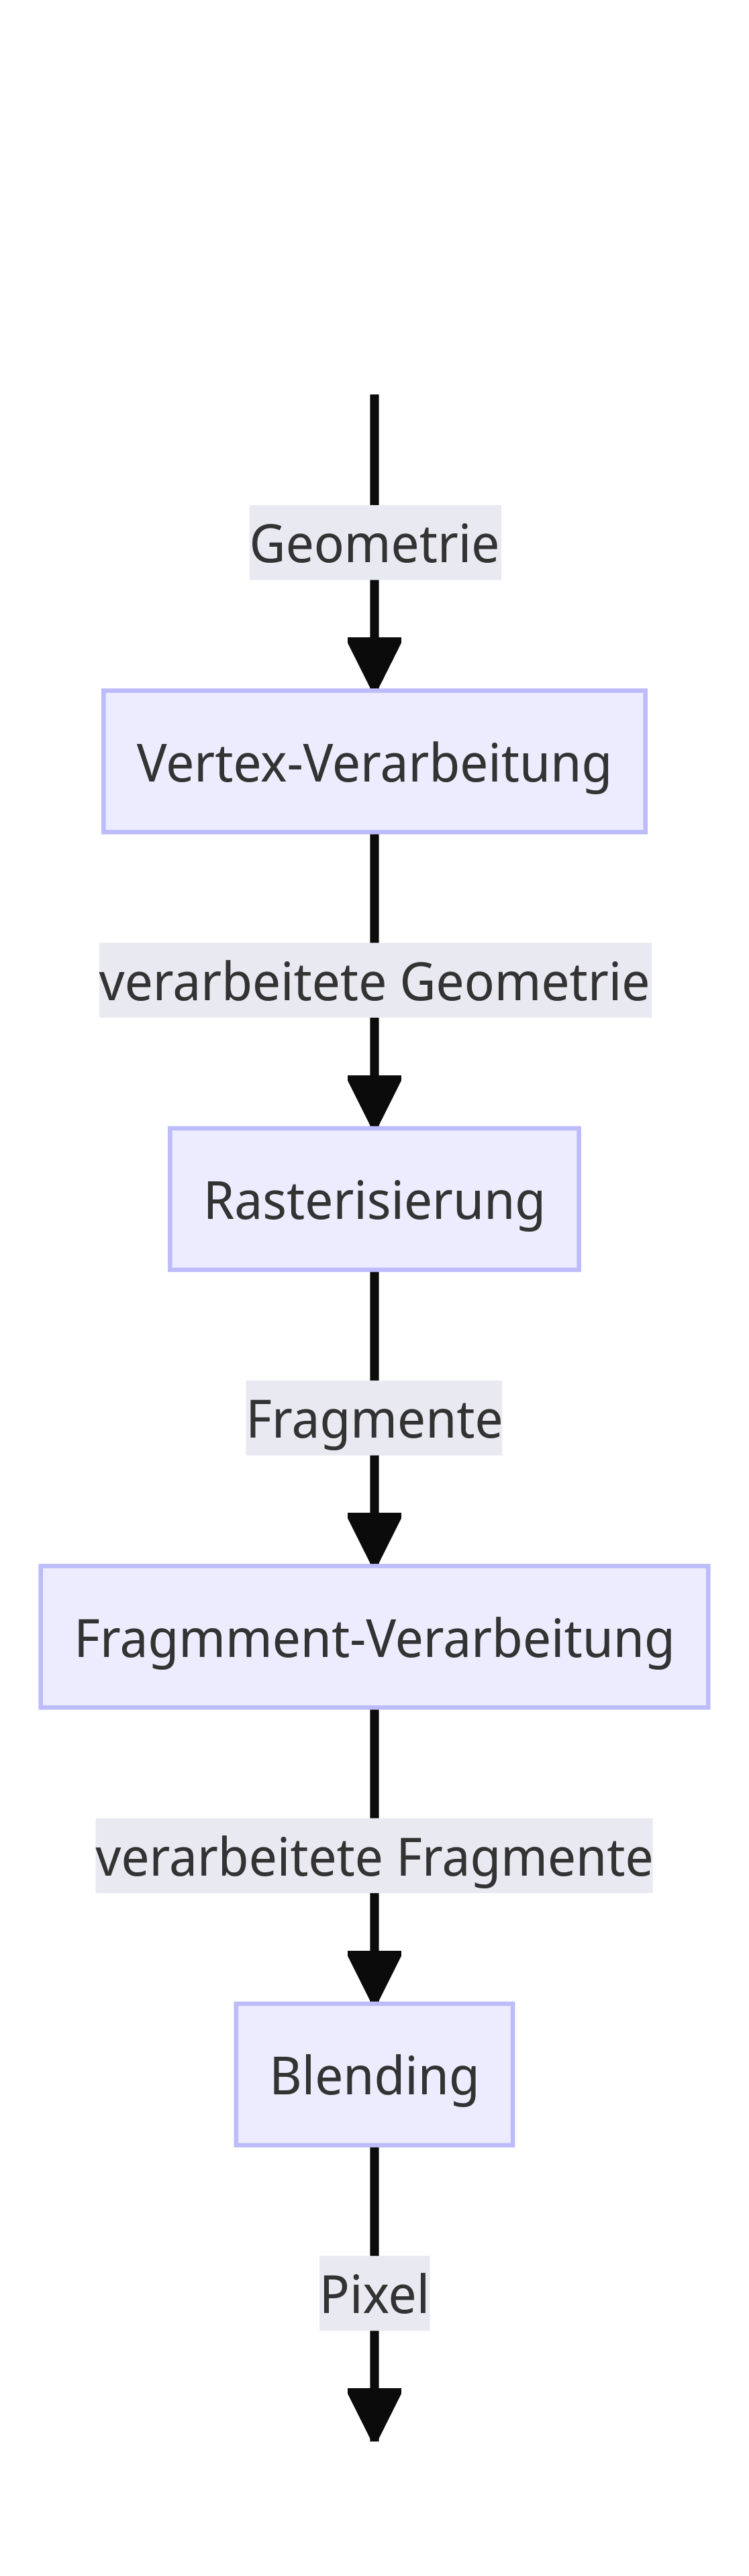
\includegraphics[width=0.5\textwidth]{../assets/img/classic_render_pipline}
            \caption{Klassisch~\autocite{visualcomputingwh-2023}}
            \label{subfig:render-pipeline-classic}
        \end{subfigure}%
        \begin{subfigure}{0.5\textwidth}
            \centering
            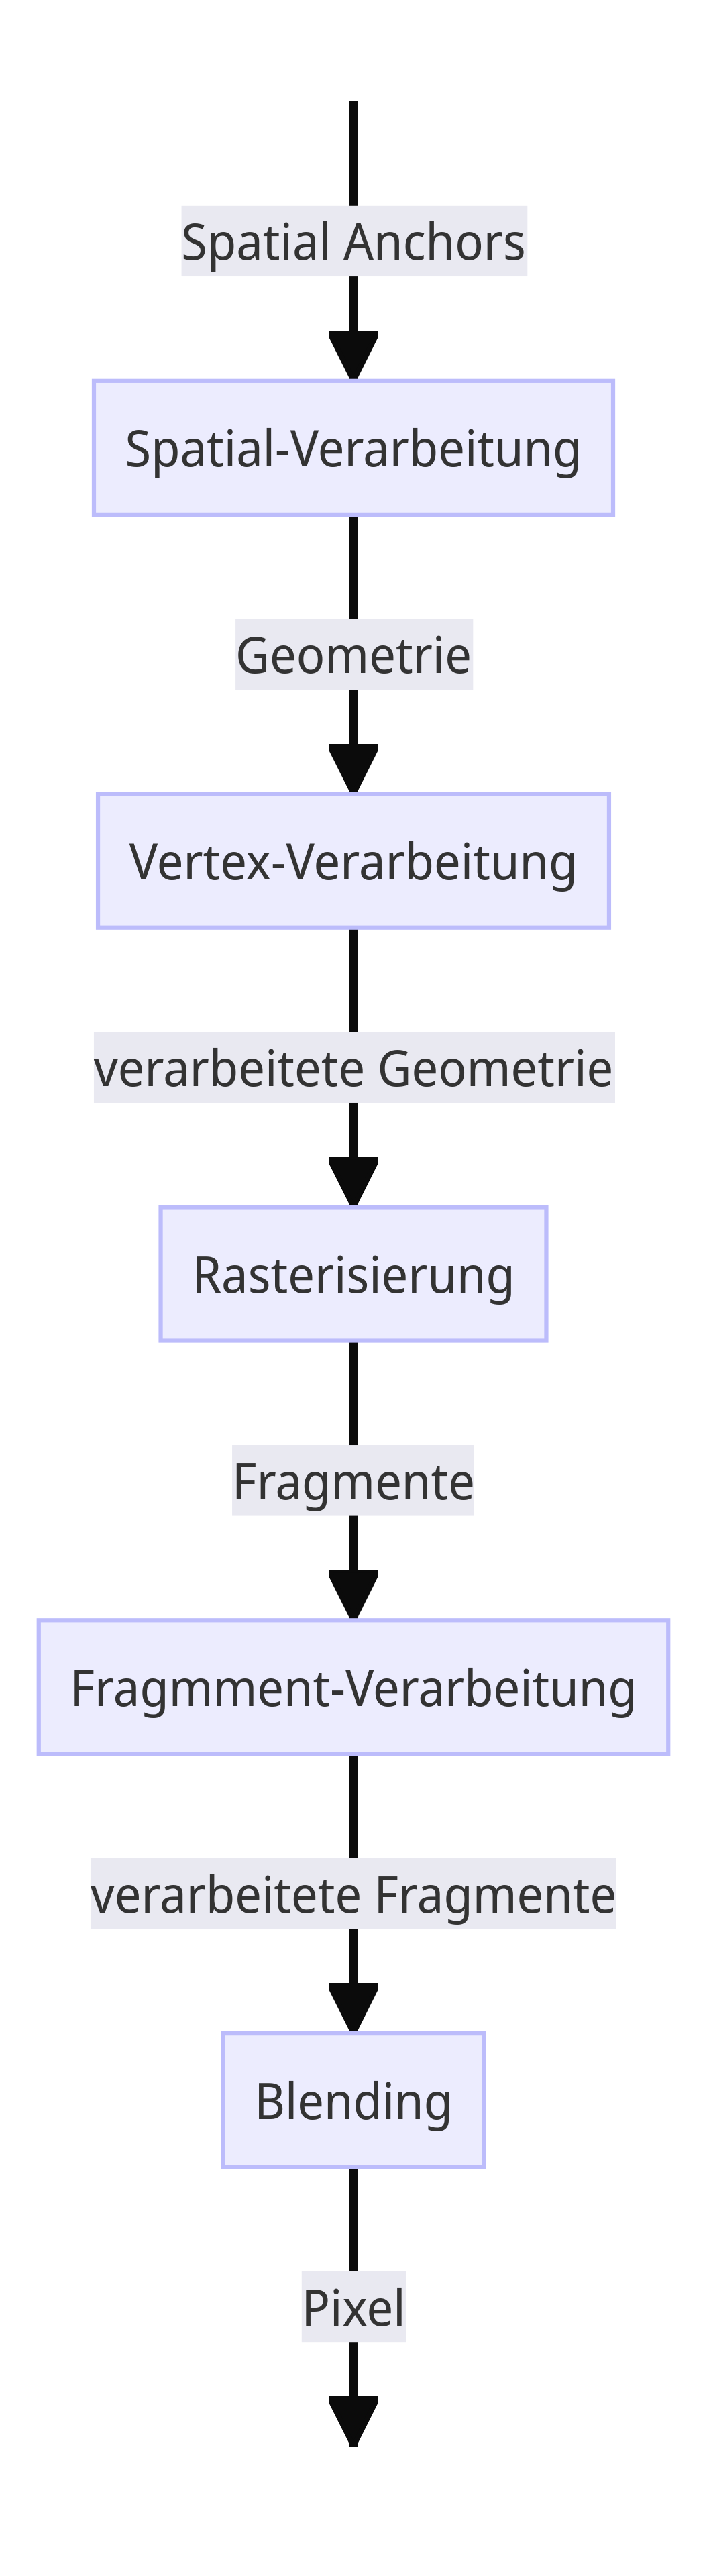
\includegraphics[width=0.5\textwidth]{../assets/img/spatial_render_pipline}
            \caption{Spatial}
            \label{subfig:render-pipeline-spatial}
        \end{subfigure}
        \caption{Render--Pipeline}
        \label{fig:render-pipeline}
    \end{figure}

    Hier findet nämlich die Transformation mittels der in \autoref{subsec:degrees-of-freedom} beschriebenen Transformationsmatrix stadt.~\autocite{visualcomputingwh-2023}

    \begin{floatingequation}[ht!]
        \begin{align}
            R_{\text{yaw}} &=&
            \begin{bmatrix}
                \cos(y_{\text{camera}}) & -\sin(y_{\text{camera}}) & 0 & 0 \\
                \sin(y_{\text{camera}}) & \cos(y_{\text{camera}})  & 0 & 0 \\
                0                       & 0                        & 1 & 0 \\
                0                       & 0                        & 0 & 1
            \end{bmatrix}\\
            R_{\text{pitch}} &=&
            \begin{bmatrix}
                \cos(p_{\text{camera}})  & 0 & \sin(p_{\text{camera}}) & 0 \\
                0                        & 1 & 0                       & 0 \\
                -\sin(p_{\text{camera}}) & 0 & \cos(p_{\text{camera}}) & 0 \\
                0                        & 0 & 0                       & 1
            \end{bmatrix}\\
            R_{\text{roll}} &=&
            \begin{bmatrix}
                1 & 0                       & 0                        & 0 \\
                0 & \cos(r_{\text{camera}}) & -\sin(r_{\text{camera}}) & 0 \\
                0 & \sin(r_{\text{camera}}) & \cos(r_{\text{camera}})  & 0 \\
                0 & 0                       & 0                        & 1
            \end{bmatrix}\\
            T_{\text{camera}} &=&
            \begin{bmatrix}
                0 & 0 & 0 & \vec{t}_{camera}\cdot\vec{e_x} \\
                0 & 0 & 0 & \vec{t}_{camera}\cdot\vec{e_y} \\
                0 & 0 & 0 & \vec{t}_{camera}\cdot\vec{e_z} \\
                0 & 0 & 0 & 1
            \end{bmatrix}
            \cdot R_{\text{yaw}}\cdot R_{\text{pitch}}\cdot R_{\text{roll}}\\
            T &=& T_{\text{Application}}\cdot T_{\text{camera}}
        \end{align}
        \caption{Transformation ohne Spatial Anchors}
        \label{eq:classic-camera-transformation}
    \end{floatingequation}

    Die Transformationsmatrix der Anwendung wird mit der inversen Transformationsmatrix des Kamera--Koordinatensystems multipliziert (Siehe \autoref{eq:classic-camera-transformation}) (und auf das klassische Sichtvolumen beschränkt,) um aus der Sicht der Kamera zu rendern.

    Für die gesamte Render--Pipeline werden dabei ausschließlich die Vertices der Objekte sowie die Transformationsmatrizen geladen.
    So müssen möglichst wenige Daten vom RAM der CPU auf den RAM der GPU übertragen werden.

    Erweitern wir diesen Prozess um Spatial Anchors so ergibt sich der Fluss aus \autoref{subfig:render-pipeline-spatial}.
    Für diese, vereinfachte, darstellung nehmen wir an, dass der stationary frame of reference ein Spatial Anchor im Uhrsprung des World Coordinate System ist.

    Effektiv benötigen in dieser neuen Phase lediglich die Transformationsmatrizen ein kleines Preprocessing, wie in \autoref{eq:spatial-camera-transformation} beschrieben.
    Bevor vom Global Coordinate System ins Camera Coordinate System transformiert wird, wird zunächst für jeden Spatial Anchor sein Koordinatensystem in das World Koordinate System überführt.

    \begin{floatingequation}[ht!]
        \begin{align}
            R_{\text{yaw}} &=&
            \begin{bmatrix}
                \cos(y_{\text{anchor}})  & \sin(y_{\text{anchor}}) & 0 & 0 \\
                -\sin(y_{\text{anchor}}) & \cos(y_{\text{anchor}}) & 0 & 0 \\
                0                        & 0                       & 1 & 0 \\
                0                        & 0                       & 0 & 1
            \end{bmatrix}\\
            R_{\text{pitch}} &=&
            \begin{bmatrix}
                \cos(p_{\text{anchor}}) & 0 & -\sin(p_{\text{anchor}}) & 0 \\
                0                       & 1 & 0                        & 0 \\
                \sin(p_{\text{anchor}}) & 0 & \cos(p_{\text{anchor}})  & 0 \\
                0                       & 0 & 0                        & 1
            \end{bmatrix}\\
            R_{\text{roll}} &=&
            \begin{bmatrix}
                1 & 0                        & 0                       & 0 \\
                0 & \cos(r_{\text{anchor}})  & \sin(r_{\text{anchor}}) & 0 \\
                0 & -\sin(r_{\text{anchor}}) & \cos(r_{\text{anchor}}) & 0 \\
                0 & 0                        & 0                       & 1
            \end{bmatrix}\\
            T_{\text{anchor}} &=&
            \begin{bmatrix}
                0 & 0 & 0 & \vec{t}_{camera}\cdot\vec{e_x} \\
                0 & 0 & 0 & \vec{t}_{camera}\cdot\vec{e_y} \\
                0 & 0 & 0 & \vec{t}_{camera}\cdot\vec{e_z} \\
                0 & 0 & 0 & 1
            \end{bmatrix}
            \cdot R_{\text{yaw}}\cdot R_{\text{pitch}}\cdot R_{\text{roll}}\\
            T &=& T_{\text{Application}}\cdot T_{\text{anchor}}\cdot T_{\text{camera}}
        \end{align}
        \caption{Transformation mit Spatial Anchors}
        \label{eq:spatial-camera-transformation}
    \end{floatingequation}

    Soweit so einfach, allerdings kommt noch hinzu, dass zunächst die Spatial Anchors ausgewertet werden müssen.
    Anhand unserer Annahme, dass es sich dabei um eine KI, oder zumindest eine Heuristik handelt, wird auch diese auf der Grafikkarte agieren.

    Aber auch dieses Problem lässt sich lösen.
    Zunächst führen wir einen Raster--Thread ein, der mit einer Rate von 30 FPS das Rendering startet.
    Im \enquote{Ruhezustand} wertet die Grafikkarte nun, mit über Zeit zunehmender Genauigkeit, die Sensordaten und damit die relativen Positionen der Spatial Anchors zueinander, aus.
    Wenn allerdings ein Frame angefordert wird, so führt die Grafikkarte einen Context--Switch durch und rendert den Frame.
    Hierzu wird zunächst ein Snapshot der Positionen der Spatial Anchors erstellt.
    Dieser wird verwendet, um die Transformationsmatrizen zu berechnen.

    Ein großes Problem, welches übrig bleibt, ist, dass die Frame--Rate für einen, sich bewegenden, Kopf noch zu langsam ist.
    Mehr leistung an den Kopf des Nutzers zu schnüren ist allerdings unpraktikabel.
    Deshalb müssen Tricks her.

    Vorteilhaft ist, dass 30 Frames für eine flüssige bewegung der Objekte in der virtuellen Umgebung reichen.
    Es muss lediglich die Bewegung des Kopfes in neuen Frames einberechnet werden.
    Zwischen den Frames wird also die verarbeitete Geometrie im RAM der GPU gelassen.
    Zusätzlich wird eine Transformationsmatrix von der vorherigen zu der aktuellen Kameraposition evaluiert und auf die Grafikkarte geladen.
    Anschließend kann damit die Render--Pipeline mit weniger Aufwand erneut durchlaufen werden.
    So können, mit wenig Aufwand, zum Beispiel 60~Frames pro Sekunde erreicht werden, auch wenn dies keine vollwertigen Frames sind.

